\section{Inference speed and memory efficiency}
\label{sec:systems}

Constant memory turns directly into serving gains. On one Hopper 80GB GPU, EdgeRock-4B decodes a single request at \textbf{\EdgeLongTPS{} tokens/s} through 128K output, runs \textbf{512} long-generation sequences at once, and averages \textbf{\EdgeBatchRatio{}$\times$} Qwen3.5-4B's end-to-end throughput. These results combine constant persistent history with CUDA Graphs and fused BF16 kernels (Appendix~\ref{app:runtime}); the same unquantized weights, BF16 KV, and FP32 recurrent state serve both single requests and concurrent batches.

\FloatBarrier
\subsection{Sustained decoding and long-generation throughput}
\label{sec:throughput}\label{sec:batch}

\paragraph{Single-request decoding.}
EdgeRock-4B sustains \textbf{\EdgeLongTPS{} tokens/s} through 128K output after 128K input, \textbf{\EdgeSingleRatio{}$\times$} Qwen3.5-4B's rate under the same workload at batch size $1$. Decoding remains nearly flat throughout generation (Figure~\ref{fig:decode-speed}a). With 254K input and 2K output, reaching the same 256K total length, EdgeRock-4B decodes at \textbf{226.6 tokens/s} versus Qwen3.5-4B's 133.9, a \textbf{1.69$\times$} gain.

\begin{figure}[!htbp]
\centering
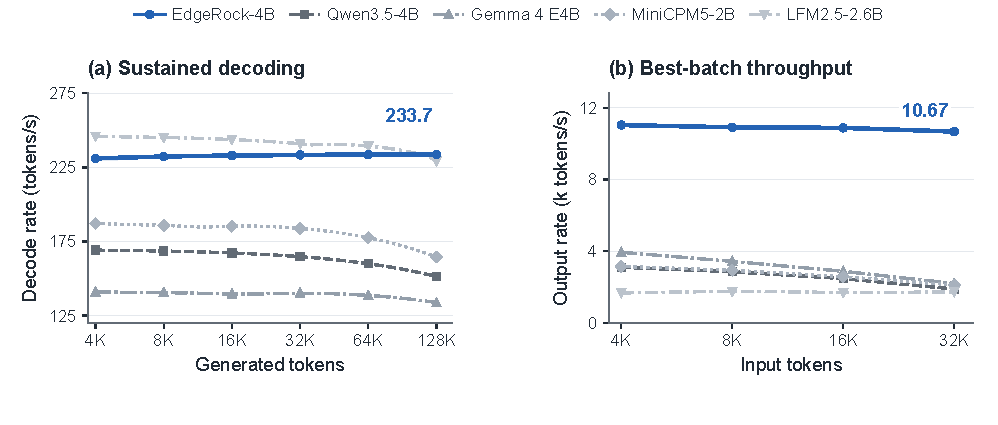
\includegraphics[width=\linewidth]{runtime_scaling.pdf}
\caption{\textbf{Long-context inference.} EdgeRock-4B and four compact models use BF16 weights and KV on one Hopper 80GB GPU; EdgeRock and Qwen use FP32 recurrent state. \textbf{(a)} Cumulative decode rate during 128K output after 128K input at batch size $1$. EdgeRock sustains \EdgeLongTPS{} tokens/s through the full output. \textbf{(b)} Output-token throughput for 4K--32K inputs and 32K output with repeated prompts. Only output tokens are counted; elapsed time includes prefill. Each model uses its best measured batch at each input length (Appendix Table~\ref{tab:peer-throughput}); EdgeRock leads across all four workloads.}
\label{fig:throughput}\label{fig:decode-speed}
\end{figure}

\paragraph{Long-generation throughput.}
Across 4K, 8K, 16K, and 32K inputs with 32K output, EdgeRock-4B averages \textbf{\EdgeBatchRatio{}$\times$} Qwen3.5-4B's end-to-end throughput and \textbf{\EdgeLFMRatio{}$\times$} LFM2.5-2.6B's at each runtime's best measured batch (Appendix Table~\ref{tab:peer-throughput}). The gain comes from capacity. At 32K input and 32K output, each Qwen3.5-4B sequence ends with 2\,GiB of attention KV (32\,KiB per token), so its cache fills after a few dozen concurrent sequences on one 80GB GPU and further requests wait. EdgeRock's persistent history stays at 121.76\,MiB per sequence, so all 512 sequences remain active through the full output.


\FloatBarrier
\subsection{Scaling concurrency and response rate}
\label{app:latency-memory}

EdgeRock-4B supports \textbf{512 concurrent sequences} across all 16 input/output combinations of 4K, 8K, 16K, and 32K tokens on one Hopper 80GB. At batch size $512$, weighted decoding reaches \textbf{\EdgeWeightedTPS{} tokens/s}, or \textbf{\EdgePerSequenceTPS{} tokens/s per active sequence}, with the same precision as single-request decoding (Figure~\ref{fig:batch-scaling}).

\begin{figure}[!htbp]
\centering
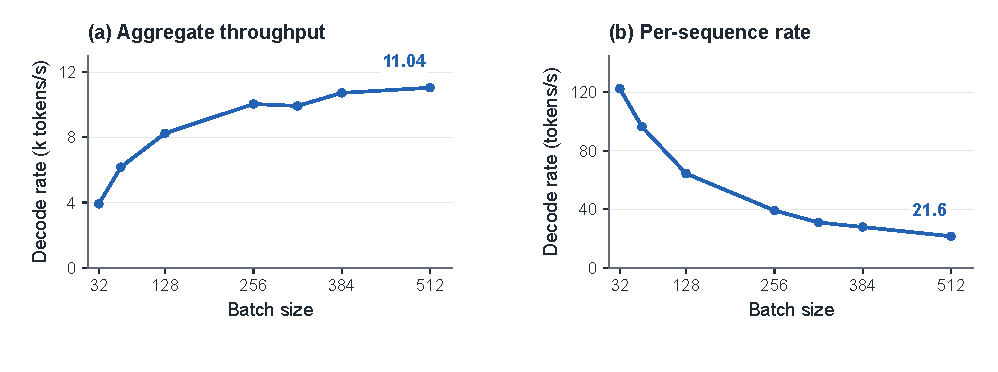
\includegraphics[width=\linewidth]{batch_scaling.pdf}
\caption{\textbf{Concurrency scaling.} EdgeRock-4B runs 32--512 active sequences on one Hopper 80GB GPU with BF16 weights, BF16 KV, and FP32 recurrence. Rates pool decode tokens and elapsed decode time across all 16 input/output pairs formed from 4K, 8K, 16K, and 32K lengths. \textbf{(a)} Aggregate throughput reaches \EdgeWeightedTPS{} tokens/s at batch size $512$. \textbf{(b)} Aggregate throughput divided by the active batch gives the mean rate per sequence: \EdgePerSequenceTPS{} tokens/s at batch size $512$.}
\label{fig:batch-scaling}
\end{figure}

\FloatBarrier
\subsection{Short-context decoding: 4K input, 2K output}
\label{sec:short}

EdgeRock-4B reaches a decode rate of \textbf{\EdgeShortTPS{} tokens/s} at batch size $1$ and \textbf{\EdgeShortBatchTPS{} tokens/s} at batch size $512$ for 4K input and 2K output, excluding prefill. At batch size $1$, peak tensor allocation is \textbf{\EdgeShortMemory{}\,GiB} (Appendix Table~\ref{tab:short-scaling}).


\FloatBarrier
\subsection{Fixed history and measured GPU memory}
\label{sec:cache}

Local attention and RMA keep history KV storage \textbf{$O(1)$ in sequence length}, with a BF16 capacity of \textbf{72\,MiB per sequence}. At 256K context, this is \textbf{99.1\% less KV} than Qwen3.5-4B's full-attention cache (Figure~\ref{fig:overview}b). Qwen3.5-4B is itself a hybrid that keeps full attention in only 8 of its 32 layers; the reduction removes the growth that this design leaves. Including FP32 recurrence and auxiliary tensors, persistent history totals \textbf{121.76\,MiB per sequence} (Table~\ref{tab:state-budget}).

A single 128K-input/128K-output request peaks at \textbf{\EdgeLongMemory{}\,GiB} of tensor allocation. At batch size $512$, the maximum across all 16 workloads is \textbf{\EdgeBatchMemory{}\,GiB}, including weights and execution workspaces (Figure~\ref{fig:memory-capacity}). History capacity depends on concurrency rather than sequence length; input/output buffers and workspace account for the remaining workload-dependent allocation. For a single request, the memory a reasoning trace needs is therefore known before it starts: weights plus 121.76\,MiB of history, whether the model reasons for 4K tokens or 256K. That predictability is what edge deployment requires when reasoning shares memory with perception.

\begin{figure}[!htbp]
\centering
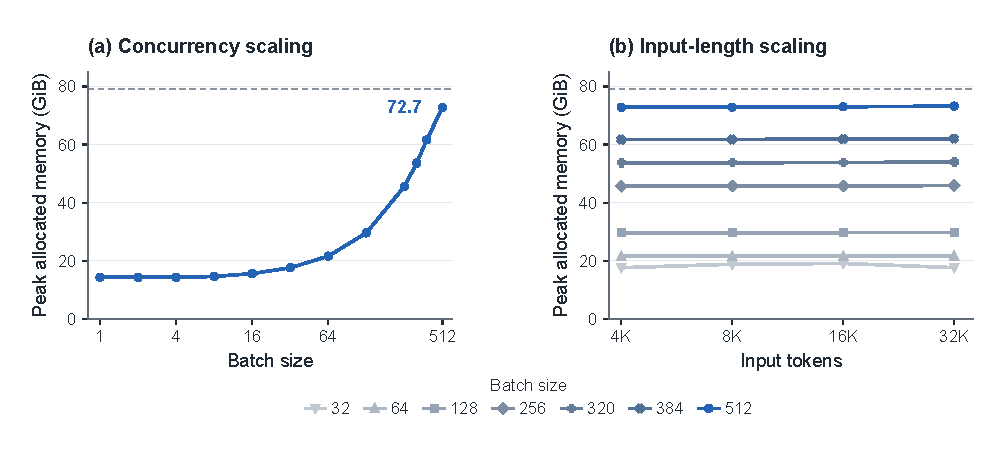
\includegraphics[width=\linewidth]{memory_capacity.pdf}
\caption{\textbf{GPU memory scaling.} EdgeRock-4B's peak tensor allocation includes model weights, persistent history, input/output buffers, and execution workspace, using BF16 weights, BF16 KV, and FP32 recurrence on one Hopper 80GB GPU. \textbf{(a)} Memory scales with concurrent requests at 4K input and 2K output. \textbf{(b)} At each fixed batch, allocation changes little as input grows from 4K to 32K with 32K output. At batch size $512$, allocation stays below 73.3\,GiB across these lengths; the dashed line marks GPU capacity.}
\label{fig:memory-capacity}
\end{figure}
